%!TEX root = ../tcc.tex

\chapter{Transmission e o BCC}
\label{chap:bcc}

Neste texto descrevemos que são encontradas vários elementos de Ciência da Computação no
programa cliente Transmission. A intensão agora é encontrar quais disciplinas da grade
curricular do Bacharelado em Ciência da Computação (BCC) da perpectiva dos conhecimentos
utilizados no Transmission.

\begin{figure}[H]
    \centering
    \fbox{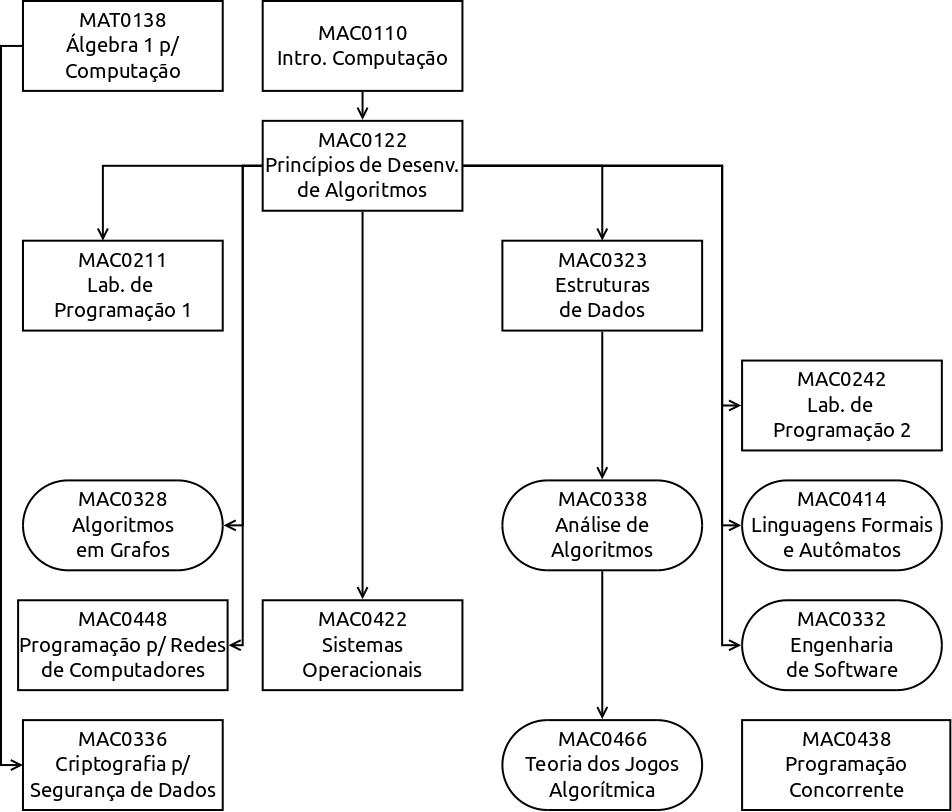
\includegraphics[width=.75\textwidth]{mapa-bcc.png}}
    \caption{disciplinas do BCC utilizadas diretamente na programação do Transmission, ligadas pelos seus pré-requisitos. As bordas arredondadas indicam que o conhecimento auxilia, mas não é necessário.}
    \label{fig:bcc}
\end{figure}

Das disciplinas do BCC, as reconhecidas como necessárias para o entendimento do
BitTorrent e o Transmission foram:

\begin{itemize}
    \item Intro. à Computação (MAC0110), Princípios de Desenvolvimento de Algoritmos
        (MAC0122), Laboratórios de Programação 1 (MAC0211): linguagem C, organização de
        código, trabalho gerenciado em grupos de desenvolvedores, portabilidade de
        código entre plataformas (Autoconf e Automake);

    \item Estruturas de Dados (MAC0323): utilização e manipulação de estruturas de
        dados, como vetores e listas ligadas;

    \item Algoritmos em Grafos (MAC0328): entendimento do algoritmo de busca de nós no
        \gls{dht};

    \item Análise de Algoritmos (MAC0328) e Teoria dos Jogos Algorítmica (MAC0446):
        algoritmo da troca das partes entre \glspl{peer};

    \item Álgebra 1 (MAT0138) e Criptografia para Segurança de Dados (MAC0336): noções
        de álgebra modular e seus usos nos métodos criptográficos;

    \item Laboratório de Programação 2 (MAC0242) e Engenharia de Software (MAC0332):
        desenvolvimento de programas complexos;

    \item Programação para Redes (MAC0448): desenvolvimento de código de conexão via
        Internet, como \gls{tcp} e \gls{udp}, multicast, \gls{nat}, IPv6, UPnP e
        \gls*{nat}-pmp;

    \item Linguagens Formais e Autômatos (MAC0414): uso de autômatos para entendimento
        dos estados dos \glspl*{peer} e suas transições com as trocas de mensagens
        \cite{conf:swarming}; e

    \item Sistemas Operacionais (MAC0422) e Programação Concorrente (MAC0438): uso de
        \glspl{thread} e métodos para computação com seus usos, como acesso à memória
        compartilhada (\emph{mutex}) e travas, e entendimento de caches de memória na
        leitura e escrita de dados.
\end{itemize}

\afterpage{\clearpage}